\documentclass[11pt,a4paper,final]{article}
\usepackage[utf8]{inputenc}
\usepackage[german]{babel}
\usepackage[T1]{fontenc}
\usepackage{amsmath}
\usepackage{amsfonts}
\usepackage{amssymb}
\usepackage[backend=biber]{biblatex}
\usepackage{gensymb}
\usepackage{graphicx}
\usepackage[onehalfspacing]{setspace}
\usepackage{url}
\usepackage{acronym}
\usepackage{minted}
%\usepackage{geometry}
%\geometry{verbose,a4paper,tmargin=25mm,bmargin=25mm,lmargin=30mm,rmargin=30mm}
\addbibresource{Bericht.bib}
\setcounter{secnumdepth}{5}
\setcounter{tocdepth}{5}

\title{\LARGE \bf
Seminararbeit\\ Architekturen und Dienste von Kommunikationsnetzen
}


\author{Frederik Wille, Julian Deinert}
\date{\today}

\begin{document}



%\maketitle
%\thispagestyle{empty}
%\pagestyle{empty}

\begin{titlepage}
	\centering
	
\includegraphics[width=0.3\textwidth]{images/uhh_logo.jpg}\hspace{1cm}
	
\includegraphics[width=0.3\textwidth]{images/tkrn_logo.jpg}\par
	{\Large Telekommunikation und Rechnernetze \\}
	{\large Fachbereich Informatik\\}
	{\large Universität Hamburg \par}
	\vspace{1.5cm}
	{\huge\bfseries Routing: Open Shortest Path First (working title)\par}
	\vspace{1.5cm}
	{\large Seminararbeit für die Lehrveranstaltung \\ \Large Architekturen und Dienste von Kommunikationsnetzen\par}

	\vfill
	\vfill
	{\Large\itshape Frederik Wille, Julian Deinert\par}

	\vfill

% Bottom of the page
	{\large \today\par}
\end{titlepage}
\thispagestyle{empty}
\newpage
\thispagestyle{empty}
\tableofcontents
\newpage
\setcounter{page}{1}

\section*{Abkürzungen}
\begin{acronym}
		\acro{igp}[IGP]{Interiour Gateway Protocol}
		\acro{egp}[EGP]{Exteriour Gateway Protocol}
		\acro{as}[AS]{Autonomous System}
		\acro{bgp}[BGP]{Border Gateway Protocol}
		\acro{ospf}[OSPF]{Open Shortest Path First}
		\acro{ip}[IP]{Internet Protocol}
		\acro{rip}[RIP]{Routing Information Protocol}
		\acro{ttl}[TTL]{Time to live}
		\acro{ack}[ACK]{Acknowledgement}
		\acro{lsdb}[LSDB]{Link-State Database}
\end{acronym}
\newpage
%%%%%%%%%%%%%%%%%%%%%%%%%%%%%%%%%%%%%%%%%%%%%%%%%%%%%%%%%%%%%%%%%%%%%%%%%%%%%%%%
\begin{abstract}
ABSTRACT

\end{abstract}

\section{Einleitung/Motivation}
% Freddy
% Layer 3
% routing vs forwarding



\section{Routing Protokolle}
\subsection{IGP und EGP}
% Freddy
Im globalem Internet werden, im Bezug auf die Beziehung zweier kommunizierenden Router, zwei Arten von Routing Protokollen verwendet. Unterschieden werden Protokolle in \ac{egp}, die zwischen zwei Netzen Routen vermitteln und \ac{igp}, die innerhalb eines Netzes das Routing übernehmen.

Die ansonsten getrennten Netze werden durch ein oder mehrere Gateways verbunden. Gateways sind Router, die zwei Netze über ein \ac{egp} verbinden. Über das \ac{egp} werden Routen zu den eigenen und auch anderen Netzen ausgetauscht. Im Internet sind Netze als Autonome Systeme organisiert, die \ac{bgp} als \ac{egp} nutzen.

Innerhalb eines Netzes müssen Routen von jedem Rechner zu jedem anderen Rechner gefunden werden. Über ein \ac{igp} tauschen die Router des Netzes die von ihnen erreichbaren Rechner aus.
Ein Rechner ist dabei immer an mindestens einem Router über ein Layer-2-Netz angebunden, das heißt mehrere Rechner können über Switches und Hubs an einen Port des Routers angeschlossen sein.

\ac{igp}s werden in zwei Klassen unterteilt, Distance-Vector- und Link-State-Protokolle.
\subsection{Distance-Vector-Routing-Protokolle}
% Freddy
Die Klasse der Distance-Vector-Protokolle setzen den Bellman-Ford-Algorithmus um. Dazu werden periodisch Arrays, auch Vektoren genannt, zu den direkten Nachbarroutern verschickt. Jeder dieser Vektoren enthält die eigenen Distanzen zu allen Zielen, die der Router zum Zeitpunkt des Sendens kennt. Dieser Distanz-Vektor gibt der Protokollklasse ihren Namen.

Zu Beginn erkennt jeder Router seine direkten Nachbarn und ermittelt die Distanz zu diesem. Aus den direkten Nachbarn wird dann ein Vektor gebildet, der dann an genau diese Nachbarn geschickt wird. Nun empfangen alle Router von ihren Nachbarn eine Reihe an Vektoren, aus denen eine Routing Tabelle gebaut werden muss. Dafür wird pro aktuell bekanntem Ziel der minimale Eintrag aller empfangener Vektoren bestimmt und als neue Distanz in die Routing Tabelle aufgenommen. Dazu wird die Adresse des Routers, von dem die Information stammt und der dazugehörige physikalische Port vermerkt. Die Herkunft wird nur lokal zum Forwarding benötigt und wird somit nicht im Vektor mitgeschickt.

Der Vorgang wird periodisch wiederholt, sodass nach und nach Routen zu allen Zielen bekannt werden. Die Tabellen der Router konvergieren über die Zeit gegen die besten Routen. Gezeigt wird dies in Abbildung~\ref{count_to_inf}a. Die benötigte Zeit kann je nach gewählter Update-Rate sehr hoch sein. Bei \ac{rip} als Beispiel wird nur alle 30 Sekunden ein Vektor verschickt. Dies führt dazu, dass bei nur 4 Routern, die in Reihe verbunden sind, bereits eine Minute für  die drei Updates\footnote{bei den Zeitpunkten 0s, 30s, 60s} benötigt wird.

Sobald ein Router ausfällt ensteht das Count-to-infinity Problem. Dabei bekommt der Nachbar des ausgefallenen Routers, eine neue Router von anderen Nachbarn, erkennt jedoch nicht, dass die Route von ihm selbst kommt.

\begin{figure}[h]
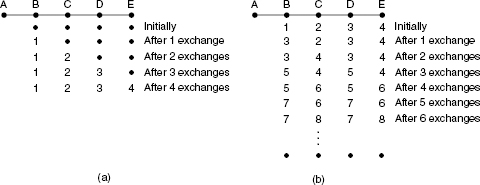
\includegraphics[width=1.0\textwidth]{images/count_to_inf.png}
\caption[count to inf]{Count to Infinity Problem\footnotemark}
\label{count_to_inf}
\end{figure}
\footnotetext{aus AndrewS.Tanenbaum2010}
Abbildung~\ref{count_to_inf}b zeigt das Count to Infinity Problem bei 5 in Reihe geschalteten Routern. Bei dem ersten Schritt ``Initially'' fällt der Knoten A aus. B bemerkt dies und bekommt beim ersten Austausch (exchange) von C einen Vektor mit der Distanz von 2 zu A. Da bei jedem Update die Tabelle komplett überschrieben werden muss, übernimmt B die neue Route mit Distanz 3 von C. Danach übernimmt C das folgende Update von B und trägt als Distanz 4 in seine Tabelle ein. Dies wiederholt sich auf allen verbliebenen Routern bis in die Unendlichkeit. Um dies abzukürzen und nicht zur höchsten vom jeweiligen Prozessor berechenbaren Zahl laufen zulassen, ist Unendlichkeit in den Protokollen definiert. Bei \ac{rip} wurde 16 gewählt. Dadurch können Routen maximal über 15 Router gehen. Es gibt mehrere Erweiterungen, die das Count-to-Infinity Problem lösen. Ein Beispiel ist Split-Horizon, bei dem genau die oben entstehende Schleife verhindert wird, indem Routen nicht an den Router, von dem sie gelernt wurden, weiter gegeben werden.

% \subsubsection{Bellman-Ford Algorithmus}
% Freddy
\subsection{Link-State-Routing-Protokolle}
Link-State-Routing-Protokolle sind eine Klasse von Routing-Protokollen, die sich dadurch auszeichnen, dass sie ihre Informationen, über die verfügbaren Routen in ihrem Netzwerk, mit all ihren Nachbarn teilen.
Im Gegensatz zu Distance-Vector-Routing-Protokollen senden sie mehrere kleine Aktualisierungen, die jeweils vollständige Routen zu andern Knoten des Netzwerks enthalten, anstatt nur Informationen über direkte Verbindungen zu ihren Nachbarknoten zu übermitteln.
Diese Informationen speichert jeder Knoten oder auch Router in einer lokalen Routing-Tabelle, die er wie folgt befüllt.

Startet ein Router in einem neuen, unbekannten Netzwerk, trägt er zunächst die Router in seine Routing-Tabelle ein, mit denen er direkt verbunden ist.
Solch ein Eintrag enthält neben der Bezeichnung des Routers auch ein Kantengewicht, welches die Verbindungsqualität zu diesem Router beschreibt.
Das Kantengewicht kann zum Beispiel die Latenz zum Nachbar-Router sein.
Dies sichert, dass dem Router bekannt ist, zu welchem anderen Router er die qualitativ beste Verbindung hat. Nachdem jeder Router all seine Nachbar-Router erkannt hat und seine lokale Routing-Tabelle aufgebaut hat, schickt dieser Link-State-Pakete an seine Nachbar-Router.
Diese Link-State-Pakete enthalten alle Nachbar-Router des Routers und die Kantengewichte zu diesen, sowie eine fortlaufende Sequenznummer und einen Zähler für das Alter des Pakets.
Jeder Router empfängt die Link-State-Pakete seiner Nachbar-Router und leitet diese an all seine Nachbar-Router weiter, die diese Pakete noch nicht erhalten haben.
Durch die Link-State-Pakete erhält jeder Router mehr Information über die Topologie des Netzwerks.
Die ankommenden Pakete werden von jedem Router in einem Paketpuffer verarbeitet.

Bei dieser Verarbeitung spielen die zwei Zähler in den Link-State-Paketen eine wichtige Rolle zur Fehlererkennung.
Diese verhindern, dass ein Router veraltete Topologie-Informationen in seine Routing-Tabelle einträgt. Dies sichert der Router, indem er nur Pakete mit der aktuell höchsten Sequenznummer annimmt.
Pakete die zwar später eingetroffen sind, jedoch eine niedrigere Sequenznummer haben, werden als veraltet behandelt und verworfen.
Eine Problematik bei diesem Vorgehen ist allerdings, dass auch Fehler in der Sequenznummer auftauchen können.
So führt ein \textit{1-bit} Fehler bei der Sequenznummer dazu, dass aus Sequenznummer 4 Sequenznummer 65540 wird.
Somit würden die Sequenznummern 5 bis 65540 als veraltete verworfen werden, bis der Router wieder neue Informationen akzeptiert.
Ein ähnliches Problem tritt auf, wenn ein Router abstürzt und mit der Sequenznummer 0 neu beginnt.
Um diesen Problemen entegegen zu wirken, enthält das Paket auch jeweils einen Alterszähler.
Dieser wird zu Beginn auf eine vordefinierte \ac{ttl} eingestellt und beispielsweise jede Sekunde um 1 dekrementiert.
Erreicht der Alterszähler den Wert 0, wird das Paket verworfen.

Nachdem ein Paket als aktuell eingestuft wurde, wird es auf allen Leitungen, ausgenommen der Leitung auf der es empfangen wurde, weitergeleitet.
Hierfür pflegt der Router innerhalb des Paketpuffers Send und \ac{ack} Flags für jeden Knoten.
Erreicht den Router ein Paket eines anderen Routers über nur eine Leitung, so wird das Send Flag bei allen anderen Leitungen gesetzt und das \ac{ack} Flag bei der Leitung gesetzt, von der das Paket kam.
Erreicht ein Paket eines anderen Routers den Router aber über zwei oder mehr unterschiedliche Leitungen, so wird auf all diesen Leitungen das \ac{ack} Flag gesetzt und das Send Flag auf den verbleibenden Leitungen.

Angeschlossen an das Befüllen der Routing-Tabelle des Routers beginnt jeder Router für sich die besten Routen durch das Netzwerk zu jedem anderen Router zu berechnen.
Hierzu nutzen Link-State-Routing Protokolle den Dijkstra-Algorithmus.
\subsubsection{Dijkstra-Algorithmus}
Der Dijkstra-Algorithmus ist ein nach seinem Erfinder Edsgar W. Dijkstra benannter Algorithmus, der in einem Graphen zu einem gegebenen Starknoten den kürzesten Pfad zu allen anderen Knoten basierend auf Kantengewichten ermittelt.

Zu Beginn werden allen Knoten des Graphens die Merkmale Distanz und Vorgänger zugewiesen. Hierbei erhält der Starknoten für die Distanz den wert $0$, die restlichen Knoten den Wert $\infty$.
Für jeden unbesuchten Knoten wird der, mit der kürzesten Distanz ausgewählt und als besucht markiert.
Zusätzlich werden für alle Nachbarknoten die Distanzen auf die Summe aus dem Distanzwert des aktuellen Knotens und dem Kantengewicht zum Nachbarknoten gesetzt.
Ergibt sich aus dem vorherigen Schritt eine niedrigere Distanz als in dem Nachbarknoten gespeichert ist, wird diese mit der niedrigeren ersetzt und der aktuelle Knoten als Vorgänger gesetzt.\\\\
\begin{minted}[
frame=lines,
framesep=3mm,
baselinestretch=1.1,
bgcolor=white,
fontsize=\footnotesize,
linenos
]{python}
def Dijkstra(Graph, source):

  create vertex set Q

  for each vertex v in Graph:       // Initialization
    dist[v] = INFINITY              // Unknown distance from source to v
    prev[v] = UNDEFINED             // Previous node in optimal path from source
    add v to Q                      // All nodes initially in Q (unvisited nodes)

  dist[source] = 0                  // Distance from source to source

  while Q is not empty:
    u = vertex in Q with min dist[u] // Source node will be selected first
    remove u from Q

    for each neighbor v of u:        // where v is still in Q.
      alt = dist[u] + length(u, v)
      if alt < dist[v]:              // A shorter path to v has been found
        dist[v] = alt
        prev[v] = u

  return dist[], prev[]
\end{minted}

\section{Open Shortest Path First}
\ac{ospf} \ac{ospf}
\subsection{Areas}
Ein \ac{ospf} Netzwerk ist häufig in sogenannte Areas aufgeteilt.
Dies schafft eine übersichtliche Struktur und erleichtert die Wartung von großen Netzwerken. In Areas werden mehrere Router zusammen gefasst und Link-State Informationen werden innerhalb der Area gespeichert und sind auch nur in ihr bekannt. 
Somit ist der interne Aufbau einer Area nach Außen hin unbekannt. 
Jede Area ist durch einen \textit{32-bit} Integer eindeutig beschrieben, der entweder als Dezimalzahl oder in Dezimalpunktschreibweise angegeben wird.
Areas sind untereinander durch einzelne Router verbunden, die an den Grenzen zwischen zwei Areas stehen, also mit beiden Areas verbunden sind.
\subsubsection{Backbone Area}
Die Area mit der Adresse 0 bzw. 0.0.0.0 wird Backbone Area genannt.
Jede andere Area muss eine direkte Verbindung zur Backbone Area haben.
Bei Ausfall eines oder mehrere Router, darf die Backbone Area nicht in mehrere Teile aufgeteilt werden.
Die Hauptaufgabe der Backbone Area besteht darin, Routing-Informationen zwischen nicht-Backbone Areas zu verteilen.
\subsubsection{Nicht-Backbone Area}
Alle an die Backbone Area angeschlossenen Areas werden nicht-Backbone Areas genannt.
Diese bestehen aus mehreren Routern, die jeweils Topologie-Informationen für ihre Area in ihrer \ac{lsdb} speichern. 
Die \ac{lsdb} ist innerhalb einer Area synchronisiert. 
\subsubsection{Stub Area}
Eine Stub Area zeichnet sich dadurch aus, dass sie keine externen Routenempfehlungen durch die Backbone Area erhält.
Weiter ist das interne Routing über Defaultrouten geregelt. Diese werden durch den mit der Backbone Area verbundenen Router verteilt, der sich selbst als Standardgateway setzt.
\subsubsection{Transit Area}
Transit Areas sind Areas, die sowohl direkt mit der Backbone Area verbunden sind, als auch mit einer nicht-Backbone Area, die selbst nicht mit der Backbone Area verbunden ist.
Da aber jede nicht-Backbone Area mit der Backbone Area verbunden sein muss, wird ein Virtual Link zur Backbone Area erstellt, der physikalisch durch die dazwischen liegende Area führt.
Diese Area bezeichnet man als Transit Area.
\subsection{Router Typen}
\subsection{Metriken}
\subsection{OSPF v2}
%julian
\subsection{OSPF v3}
%julian
\section{Fazit/Ausblick}
Julian

\clearpage
\nocite{*}
\printbibliography
\end{document}
